\documentclass[a4paper, 12pt]{article}

\usepackage[utf8]{inputenc}
\usepackage[T2A]{fontenc}
\usepackage[english, russian]{babel}

\usepackage{enumitem}
\setlist{nolistsep}
\usepackage{mathtools}
\usepackage{xcolor}
\definecolor{dimblue}{HTML}{1010aa}
\usepackage[
	colorlinks=true, 
	allcolors=dimblue
]{hyperref}
\usepackage[
	vmargin=1in,
	hmargin=1in
]{geometry}
\linespread{1.3}
\usepackage{indentfirst}
\usepackage{graphicx}
\usepackage[multidot]{grffile}
\usepackage[labelsep=period]{caption}


\begin{document}

\noindent
Гусейнов Керим Демирович, физический факультет
\hfill
9 декабря 2020

\begin{center}
	\textbf{12. События Дансгора-Оешгера}
\end{center}

Изменения климата Земли известно с все меньшей точностью при удалении 
от настоящего времени в прошлое, в результате чего имеется некая 
матрешечная картина. При рассмотрении событий на разных временных 
интервалах видны разные колебания и прослеживаются разные явления. То 
есть физика процессов, обуславливающих события в рамках тысячелетий 
и в рамках миллионов лет, естественно, не одна и та же. В связи с этим, 
принято рассматривать временные отрезки разной величины по отдельности.

Последняя эпоха оледенения длилась примерно с 120 до 20 тысяч лет 
назад и, поскольку находится ближе всего к настоящему моменту, 
известна наиболее подробно. Вариации климата за этот промежуток 
времени, определенные по ледниковым кернам Антарктиды и Гренландии, 
представлены на рисунке~\ref{fig:last}. Как видно, общее похолодание 
не является постоянным, а прерывается довольно сильными и резкими 
периодами потепления, которые и называют событиями Дансгора-Оешгера. 
Размах соответствующих колебаний близок к наблюдаемому при переходе 
от ледниковой стадии к межледниковью. Иногда события ДЭ следовали 
одно за другим, а иногда оказывались изолированными. Источником этих 
событий является путешествие водных массивов в океанах, а именно -- 
в северной Атлантике. Гольфстрим, поднимаясь на север вдоль Америки, 
опускается в Норвежском море благодаря как температуре, так 
и солености. Пришедшая из океана вода при охлаждении начинает тонуть 
и накапливаться подо льдом. Через какое-то время она переливается 
через подводный рельеф и течет под водой, путешествуя по океанам. 
Вода всплывает в Тихом океане, затем в Индийском, а затем 
возвращается обратно. Общий период процесса составляет порядка 
400~лет. Таким образом, события ДЭ это появление более пресных вод 
и остановка конвекции. Теплая вода в этом случае идет на меньшие 
широты, охлаждается на севере, а по мере ее перемещения, постепенно, 
все широты оказываются затронутыми.

\begin{figure}[b!]
	%\vskip-5\baselineskip
	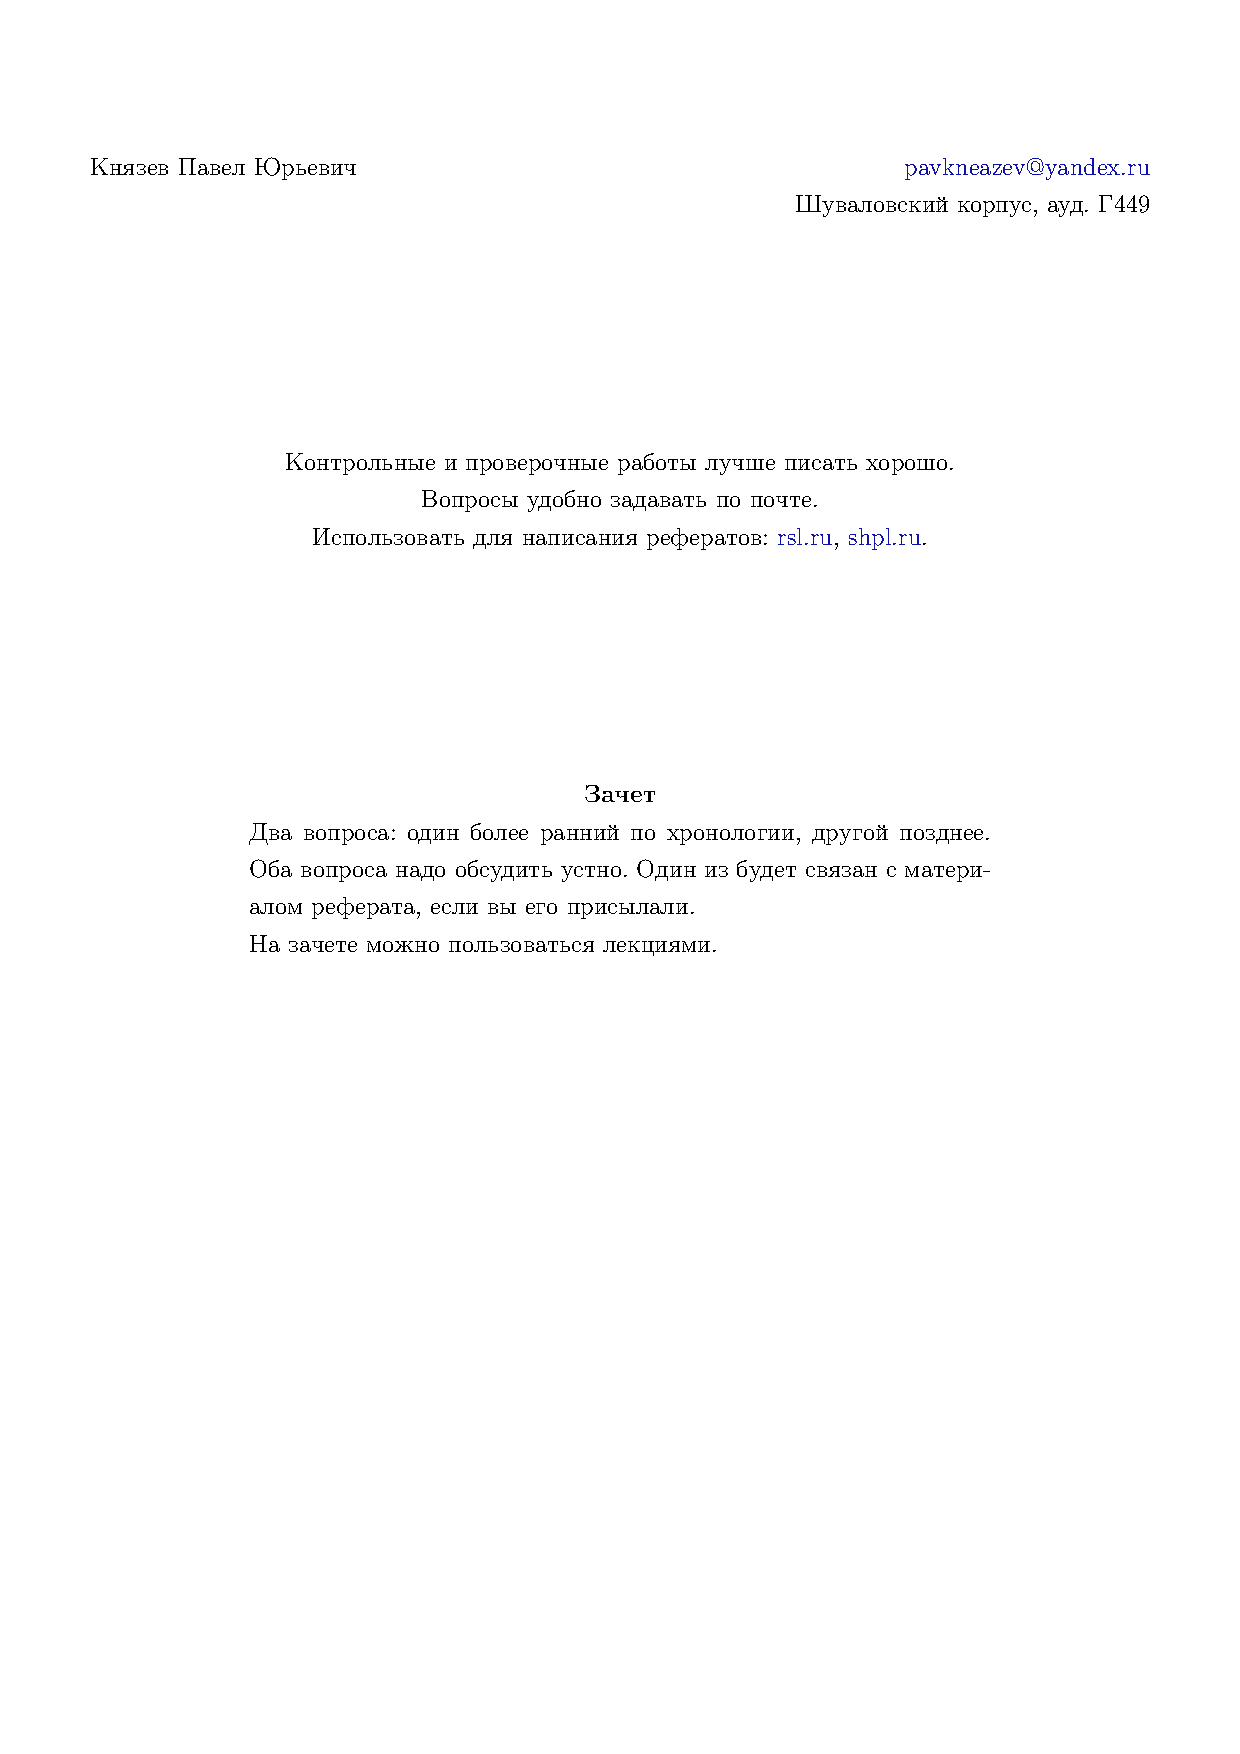
\includegraphics[height=\linewidth, origin=c, angle=271]{/home/kerim/Pictures/history.pdf}
	\vskip-5\baselineskip
	\caption{Изменение температуры на Земле за последние 0.54 млрд. лет.}
	\label{fig:history}
\end{figure}

\begin{figure}[b!]
	\includegraphics[width=\linewidth]{/home/kerim/Pictures/last140k.pdf}
	\caption{Вариации климата по данным о динамике дейтерия по данным 
	керна Восток в Антарктиде (а) и динамике содержания изотопа 
	тяжелого кислорода в составе молекул воды по данным ледяных кернов 
	Гренландии (б).}
	\label{fig:last}
\end{figure}


\end{document}
